\chapter*{Введение}                         % Заголовок
\addcontentsline{toc}{chapter}{Введение}    % Добавляем его в оглавление, если нет нумерации, то есть
%\chapter*{Введение}

\newcommand{\actuality}{}
\newcommand{\progress}{}
\newcommand{\aim}{{\textbf\aimTXT}}
\newcommand{\tasks}{\textbf{\tasksTXT}}
%\newcommand{\novelty}{\textbf{\noveltyTXT}}
\newcommand{\influence}{\textbf{\influenceTXT}}
\newcommand{\methods}{\textbf{\methodsTXT}}
\newcommand{\defpositions}{\textbf{\defpositionsTXT}}
\newcommand{\reliability}{\textbf{\reliabilityTXT}}
\newcommand{\probation}{\textbf{\probationTXT}}
\newcommand{\contribution}{\textbf{\contributionTXT}}
\newcommand{\publications}{\textbf{\publicationsTXT}}

%\input{common/characteristic} % Характеристика работы по структуре во введении и в автореферате не отличается (ГОСТ Р 7.0.11, пункты 5.3.1 и 9.2.1), потому её загружаем из одного и того же внешнего файла, предварительно задав форму выделения некоторым параметрам

%\textbf{Объем и структура работы.} Диссертация состоит из~введения, трёх глав,
%заключения и~двух приложений.
%% на случай ошибок оставляю исходный кусок на месте, закомментированным
%Полный объём диссертации составляет  \ref*{TotPages}~страницу
%с~\totalfigures{}~рисунками и~\totaltables{}~таблицами. Список литературы
%содержит \total{citenum}~наименований.
%
%Полный объём диссертации составляет
%\formbytotal{TotPages}{страниц}{у}{ы}{}, включая
%\formbytotal{totalcount@figure}{рисун}{ок}{ка}{ков} и
%\formbytotal{totalcount@table}{таблиц}{у}{ы}{}.   Список литературы содержит
%\formbytotal{citenum}{наименован}{ие}{ия}{ий}.

\noindent

\begin{figure}[!h]
	\centering
  \tikzset{every picture/.style={line width=0.75pt}} %set default line width to 0.75pt
  
  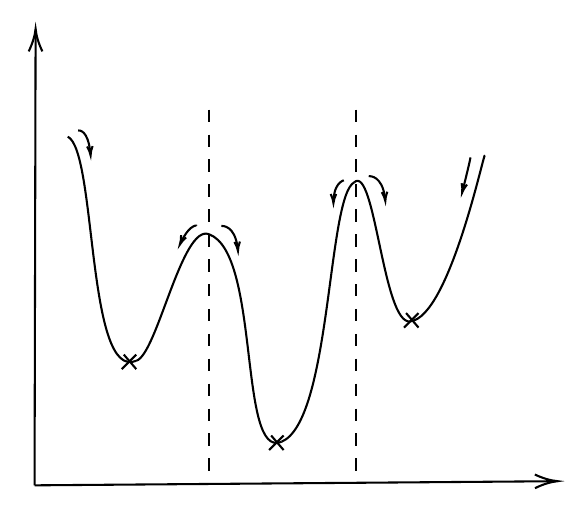
\begin{tikzpicture}[x=0.75pt,y=0.75pt,yscale=-1,xscale=1]
  %uncomment if require: \path (0,739); %set diagram left start at 0, and has height of 739

  %Curve Lines [id:da37232558430014473]
  \draw    (133.5,110) .. controls (158.5,119) and (147.5,219) .. (168.5,210) ;
  %Straight Lines [id:da3476897261424843]
  \draw    (49.5,231) -- (50,13) ;
  \draw [shift={(50,11)}, rotate = 450.13] [color={rgb, 255:red, 0; green, 0; blue, 0 }  ][line width=0.75]    (10.93,-3.29) .. controls (6.95,-1.4) and (3.31,-0.3) .. (0,0) .. controls (3.31,0.3) and (6.95,1.4) .. (10.93,3.29)   ;
  %Straight Lines [id:da355319366378235]
  \draw    (49.5,231) -- (299.5,229.02) ;
  \draw [shift={(301.5,229)}, rotate = 539.55] [color={rgb, 255:red, 0; green, 0; blue, 0 }  ][line width=0.75]    (10.93,-3.29) .. controls (6.95,-1.4) and (3.31,-0.3) .. (0,0) .. controls (3.31,0.3) and (6.95,1.4) .. (10.93,3.29)   ;
  %Curve Lines [id:da9451459693396738]
  \draw    (98.5,171) .. controls (108.5,168) and (120.5,105) .. (133.5,110) ;
  %Curve Lines [id:da9118683996504104]
  \draw    (168.5,210) .. controls (192.5,200) and (190.5,92) .. (203.5,85) ;
  %Curve Lines [id:da2198725124040073]
  \draw    (98.5,171) .. controls (74.5,181) and (79.5,70) .. (65.5,63) ;
  %Curve Lines [id:da7607618362532125]
  \draw    (230.5,152) .. controls (217.5,154) and (213.5,76) .. (203.5,85) ;
  %Curve Lines [id:da5694398882679776]
  \draw    (266.5,72) .. controls (266.5,68) and (249.5,150) .. (230.5,152) ;
  %Straight Lines [id:da9091864738783852]
  \draw  [dash pattern={on 4.5pt off 4.5pt}]  (133.5,50) -- (133.5,230) ;
  %Straight Lines [id:da6947024773973995]
  \draw  [dash pattern={on 4.5pt off 4.5pt}]  (204.5,50) -- (204.5,230) ;
  %Curve Lines [id:da3791802319426323]
  \draw [line width=0.75]    (70.5,60) .. controls (71.45,60) and (75.07,60) .. (76.31,70.13) ;
  \draw [shift={(76.5,72)}, rotate = 265.24] [color={rgb, 255:red, 0; green, 0; blue, 0 }  ][line width=0.75]    (4.37,-1.32) .. controls (2.78,-0.56) and (1.32,-0.12) .. (0,0) .. controls (1.32,0.12) and (2.78,0.56) .. (4.37,1.32)   ;
  %Curve Lines [id:da6195588467790258]
  \draw [line width=0.75]    (127.5,106) .. controls (128.45,106) and (124.92,104.21) .. (120.32,113.3) ;
  \draw [shift={(119.5,115)}, rotate = 294.44] [color={rgb, 255:red, 0; green, 0; blue, 0 }  ][line width=0.75]    (4.37,-1.32) .. controls (2.78,-0.56) and (1.32,-0.12) .. (0,0) .. controls (1.32,0.12) and (2.78,0.56) .. (4.37,1.32)   ;
  %Curve Lines [id:da14497801079245498]
  \draw [line width=0.75]    (139.5,106) .. controls (140.45,106) and (145.86,106) .. (147.29,116.13) ;
  \draw [shift={(147.5,118)}, rotate = 265.24] [color={rgb, 255:red, 0; green, 0; blue, 0 }  ][line width=0.75]    (4.37,-1.32) .. controls (2.78,-0.56) and (1.32,-0.12) .. (0,0) .. controls (1.32,0.12) and (2.78,0.56) .. (4.37,1.32)   ;
  %Curve Lines [id:da9889620169568767]
  \draw [line width=0.75]    (198.5,84) .. controls (199.44,84) and (194.19,84) .. (193.56,93.14) ;
  \draw [shift={(193.5,95)}, rotate = 270] [color={rgb, 255:red, 0; green, 0; blue, 0 }  ][line width=0.75]    (4.37,-1.32) .. controls (2.78,-0.56) and (1.32,-0.12) .. (0,0) .. controls (1.32,0.12) and (2.78,0.56) .. (4.37,1.32)   ;
  %Curve Lines [id:da9629769567992466]
  \draw [line width=0.75]    (210.5,82) .. controls (211.45,82) and (216.86,82) .. (218.29,92.13) ;
  \draw [shift={(218.5,94)}, rotate = 265.24] [color={rgb, 255:red, 0; green, 0; blue, 0 }  ][line width=0.75]    (4.37,-1.32) .. controls (2.78,-0.56) and (1.32,-0.12) .. (0,0) .. controls (1.32,0.12) and (2.78,0.56) .. (4.37,1.32)   ;
  %Curve Lines [id:da8600369809168591]
  \draw [line width=0.75]    (259.5,73) .. controls (259.5,73.87) and (257.23,83.07) .. (255.98,88.08) ;
  \draw [shift={(255.5,90)}, rotate = 284.04] [color={rgb, 255:red, 0; green, 0; blue, 0 }  ][line width=0.75]    (4.37,-1.32) .. controls (2.78,-0.56) and (1.32,-0.12) .. (0,0) .. controls (1.32,0.12) and (2.78,0.56) .. (4.37,1.32)   ;
  %Straight Lines [id:da8419867407870811]
  \draw    (92.5,168) -- (98.5,175) ;
  %Straight Lines [id:da60250082383082]
  \draw    (91.5,175) -- (98.5,168) ;
  %Straight Lines [id:da2923147725897497]
  \draw    (163.5,207) -- (169.5,214) ;
  %Straight Lines [id:da6189752522449852]
  \draw    (162.5,214) -- (169.5,207) ;
  %Straight Lines [id:da7981501034400449]
  \draw    (228.5,148) -- (234.5,155) ;
  %Straight Lines [id:da623222829834631]
  \draw    (227.5,155) -- (234.5,148) ;
  \end{tikzpicture}
	\label{img:example}
\end{figure}
